\chapter{Case Study}
\label{chap:casestudy}

%of the system: Class diagrams (components), ER, algorithms if there are any

%%%%%%%%%%%%%%%%%%%%%%%%%%%%%%%%%%%%%%%%%%%%%%%%%%%%%%%%%%%%%%%%%%%%%%%%%
\section{System Architecture}
\label{sec:sysarch}
%%%%%%%%%%%%%%%%%%%%%%%%%%%%%%%%%%%%%%%%%%%%%%%%%%%%%%%%%%%%%%%%%%%%%%%%%


%%%%%%%%%%%%%%%%%%%%%%%%%%%%%%%%%%%%%%%%%%%%%%%%%%%%%%%%%%%%%%%%%%%%%%%%%
\section{Entity Type Relation}
\label{sec:enttyperelation}
%%%%%%%%%%%%%%%%%%%%%%%%%%%%%%%%%%%%%%%%%%%%%%%%%%%%%%%%%%%%%%%%%%%%%%%%%


%%%%%%%%%%%%%%%%%%%%%%%%%%%%%%%%%%%%%%%%%%%%%%%%%%%%%%%%%%%%%%%%%%%%%%%%%
\section{User Interface Diagram}
\label{sec:uidiagram}
%%%%%%%%%%%%%%%%%%%%%%%%%%%%%%%%%%%%%%%%%%%%%%%%%%%%%%%%%%%%%%%%%%%%%%%%%

%%%%%%%%%%%%%%%%%%%%%%%%%%%%%%%%%%%%%%%%%%%%%%%%%%%%%%%%%%%%%%%%%%%%%%%%%
\section{Design Methodology}
\label{sec:designmethodology}
%%%%%%%%%%%%%%%%%%%%%%%%%%%%%%%%%%%%%%%%%%%%%%%%%%%%%%%%%%%%%%%%%%%%%%%%%

On the left list we should have all organizational context definitions and on the right one only ones that are contained in an informal process. The dropdown box of the initial and final context defines the selection inside of an informal process, thus right side.

So, in db.cljs, we should have only a list of context definitions no :initial-contexts and :desired-final-contexts. Only :organizational-contexts and under this all available contexts. Under the left list, we present these elements. Right list should refer to the initial-context, final-contexts, etc. of the informal process model depending on the selection of the dropbox button. For instance if we have initial contexts selected on the dropdown box, we should present the initial contexts in the right list.

I have changed the code accordingly and provided you an example how you should change data from views.cljs. All data should be stored in db.cljs. This applies to the text fields of all elements. Whenever, we want to update something we need to update the map in db.cljs and this will be propagated to the views.


On the left side of each list item, you should present all available items of context definitions or intentions whatever type is selected there. On the right side only the ones contained in the respective informal process model. Inside of another entity, you should refer to other entities using their ids and these ids should be resolved using, for instance, intentions vector. You check each intention in the intentions vector, if it’s id is the same as the id you are looking for it, you found it and you use the information about it.  


Please align it with the structure and names of the IPSM.xsd. Each variableName like this is written like variable-name. Each complex type is a map each attribute is a key value pair and each element in another element is another key value pair.

\begin{Listing}
	\begin{lstlisting}
:entity-data {:informal-process-definitions [IPD1 IPD2]
	          :context-definitions [CTX1 CTX2 CTX3]
	          :intentions [INT1 INT2]} 
	\end{lstlisting}
	\caption{Entity data definition inside db.cljs}
	\label{lst:entitydatalist}
\end{Listing}

\section{Realization of Intention-centric Organizational Modeling}
\label{sec:realization}
%how did I implement, technology and frameworks used and why.

\hspace{4ex} This chapter discusses about how Intention-centric organizational modeling realized as an user interface editor. This also explains the realization of requirements described in Chapter 4. In the first section, we will first discuss the overview of basic concepts and then specify the design components required for the realization of this editor. The next section discusses about how the entity views in particular are realized. The last section covers in detail how individual requirement has been realized through the web editor.


%%%%%%%%%%%%%%%%%%%%%%%%%%%%%%%%%%%%%%%%%%%%%%%%%%%%%%%%%%%%%%%%%%%%%%%%%
\subsection{Basic Concepts}
\label{subsec:basicconcepts}
%%%%%%%%%%%%%%%%%%%%%%%%%%%%%%%%%%%%%%%%%%%%%%%%%%%%%%%%%%%%%%%%%%%%%%%%%
\hspace{4ex} The basic concepts section provides an overview about the architectural details like design patterns and frameworks of the developed web editor.


%%%%%%%%%%%%%%%%%%%%%%%%%%%%%%%%%%%%%%%%%%%%%%%%%%%%%%%%%%%%%%%%%%%%%%%%%
\subsection{Specifications}
\label{subsec:specifications}
%%%%%%%%%%%%%%%%%%%%%%%%%%%%%%%%%%%%%%%%%%%%%%%%%%%%%%%%%%%%%%%%%%%%%%%%%
In order to realize the web editor of Intention-centric Organizational Modeling, a formal inquiry has been done and concluded with the below specifications.

\begin{enumerate}   
	\item \textbf{Clojurescript} as the programming language
	\item \textbf{IntelliJIDEA} as the IDE
	\item \textbf{MVC} as the architecture pattern
	\item \textbf{Re-frame} as the pattern for writing SPAs in ClojureScript, using Reagent	
\end{enumerate}

%%%%%%%%%%%%%%%%%%%%%%%%%%%%%%%%%%%%%%%%%%%%%%%%%%%%%%%%%%%%%%%%%%%%%%%%%
\subsection{MVC Architecture}
\label{subsec:mvcarch}
%%%%%%%%%%%%%%%%%%%%%%%%%%%%%%%%%%%%%%%%%%%%%%%%%%%%%%%%%%%%%%%%%%%%%%%%%
\hspace{4ex} The architecture of the UI editor is based on the \textbf{Model-View-Control (MVC)} design pattern. The MVC paradigm allows to separate business logic from the code that controls presentation and event handling \cite{Oracle2016}.Each entity view in the web page is made up of combination of at least on Model and View, and one or more Controls. The individual files which acts an Model, View and Controller has been shown in the Figure \ref{fig:mvc_arch}

\begin{itemize}
	\item \textbf{Model} artifact stores the required data structure for web-editor. In the developed model artifact, the four main types of data stored inside the artifact are intentions, strategies, capabilities and informal process instances. 
	\item \textbf{View} artifact contains HTML elements and HTML constructs that describe the way of displaying the data from Model to the user.
	\item \textbf{Control} artifact contains the handler functions which can only change the model. Even the initial values of the model are put inside the control. 
\end{itemize}


\begin{figure}
	\centering
	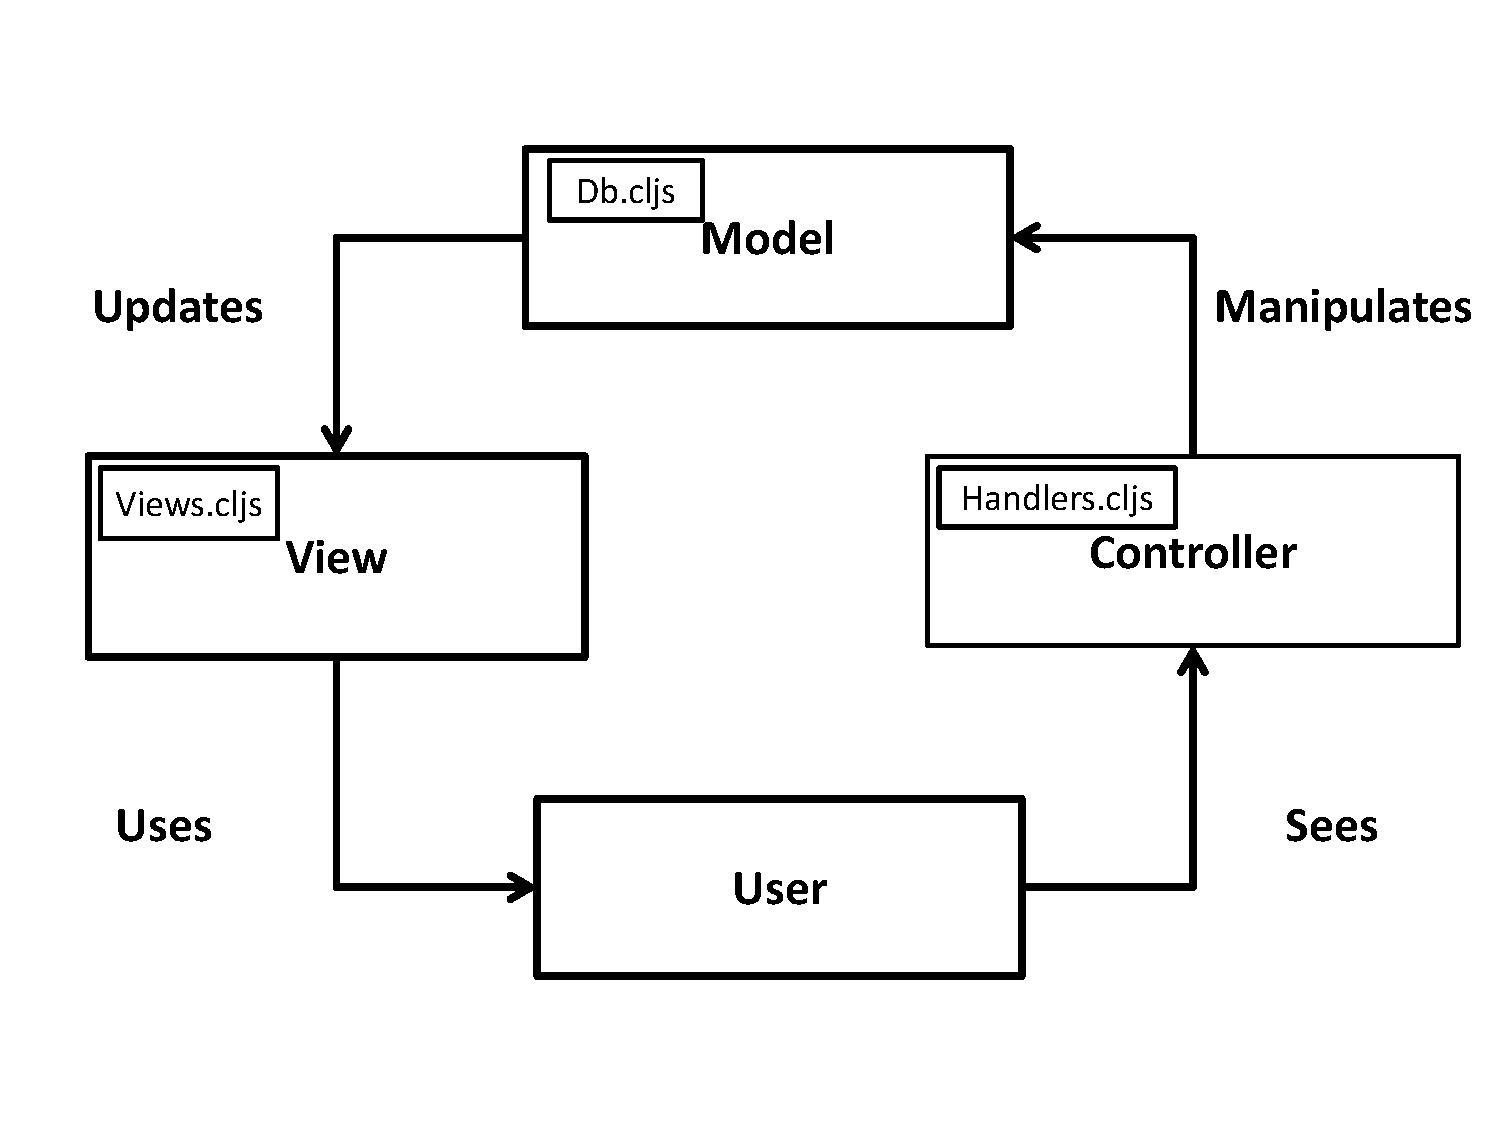
\includegraphics [width= 0.75\textwidth]{mvc_arch.pdf}
	\caption{Relationship between developed web editor artifacts and MVC architecture components}
	\label{fig:mvc_arch}
\end{figure}


%%%%%%%%%%%%%%%%%%%%%%%%%%%%%%%%%%%%%%%%%%%%%%%%%%%%%%%%%%%%%%%%%%%%%%%%%
\subsubsection{Example: Component using MVC Pattern }
%%%%%%%%%%%%%%%%%%%%%%%%%%%%%%%%%%%%%%%%%%%%%%%%%%%%%%%%%%%%%%%%%%%%%%%%%
\hspace{4ex} The Figure \ref{fig:mvc_arch} below shows the simplifed version of how the components interact with each other using the Model-View-Control (MVC) pattern, for the functionality adding new entity data. This functionality is same for all the types intentions, strategies, capabilities and informal proceess instances and below is the detailed explanation of each interaction.

\begin{enumerate}
	\item User clicks the tab \textbf{Add New} in the web editor.
	\item View, in response to the user click displays the UI component for entering the new entity data details.
	\item User enters the required basic details for adding new entity data and clicks save button.
	\item View dispatches the data to Control, which can only modify the Model.
	\item Control inserts/updates data into the model.
	\item View displays the updated model as it has been subscribed to the model.
\end{enumerate}

\begin{figure}
	\centering
	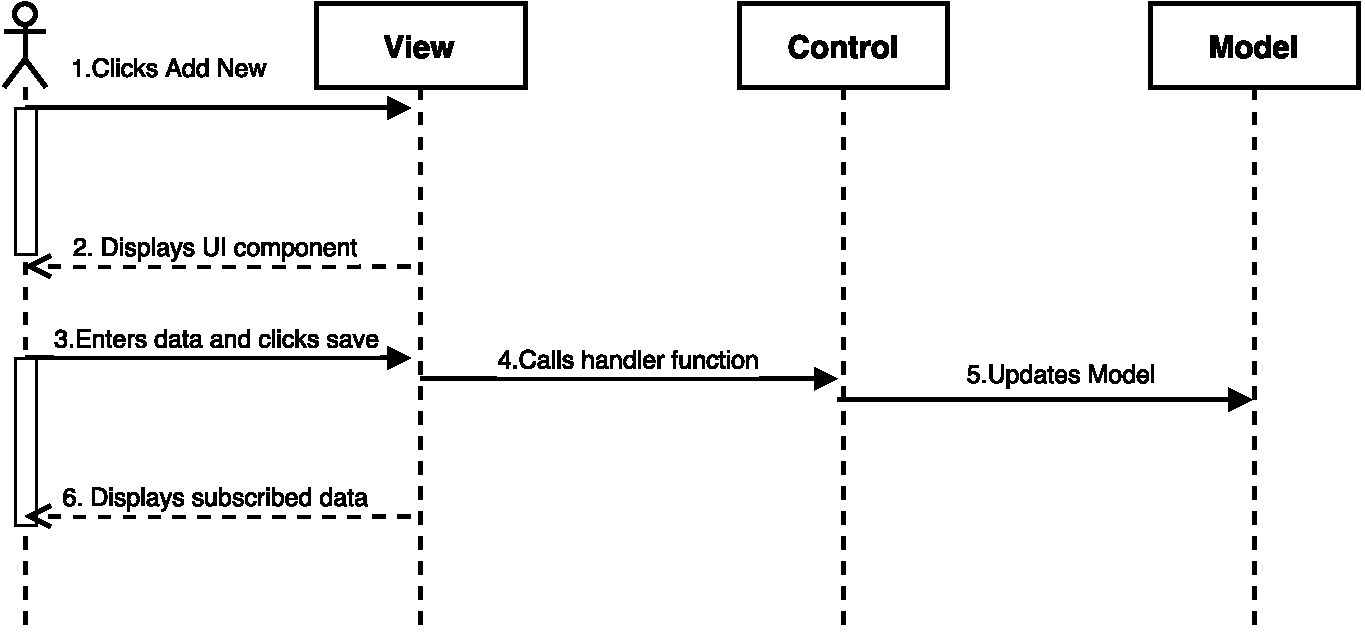
\includegraphics [width= \textwidth]{mvc_pattern.pdf}
	\caption{MVC Pattern of adding new entity}
	\label{fig:mvc_pattern}
\end{figure}
%%%%%%%%%%%%%%%%%%%%%%%%%%%%%%%%%%%%%%%%%%%%%%%%%%%%%%%%%%%%%%%%%%%%%%%%%
\subsection{Flux Architecture}
\label{subsec:fluxarch}
%%%%%%%%%%%%%%%%%%%%%%%%%%%%%%%%%%%%%%%%%%%%%%%%%%%%%%%%%%%%%%%%%%%%%%%%%

\cite{Flux2016}

\begin{figure}
	\centering
	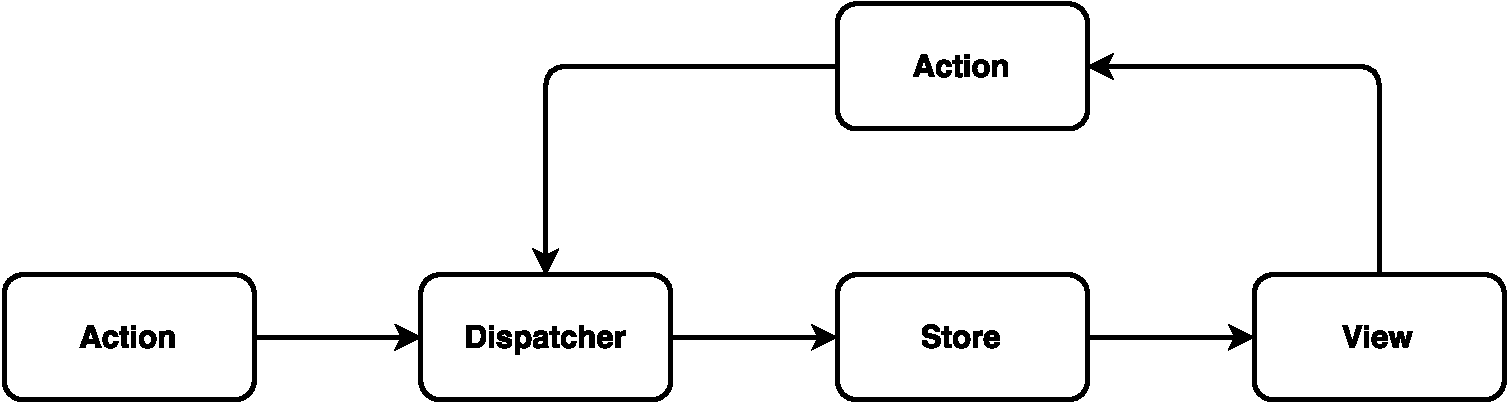
\includegraphics [width= \textwidth]{flux_arch.pdf}
	\caption{Flux Architecture \cite{Flux2016}}
	\label{fig:flux_arch}
\end{figure}

%%%%%%%%%%%%%%%%%%%%%%%%%%%%%%%%%%%%%%%%%%%%%%%%%%%%%%%%%%%%%%%%%%%%%%%%%
\subsection{Using Reagent Framework}
\label{subsec:reagent}
%%%%%%%%%%%%%%%%%%%%%%%%%%%%%%%%%%%%%%%%%%%%%%%%%%%%%%%%%%%%%%%%%%%%%%%%%

\cite{Reframe2016}

\begin{figure}
	\centering
	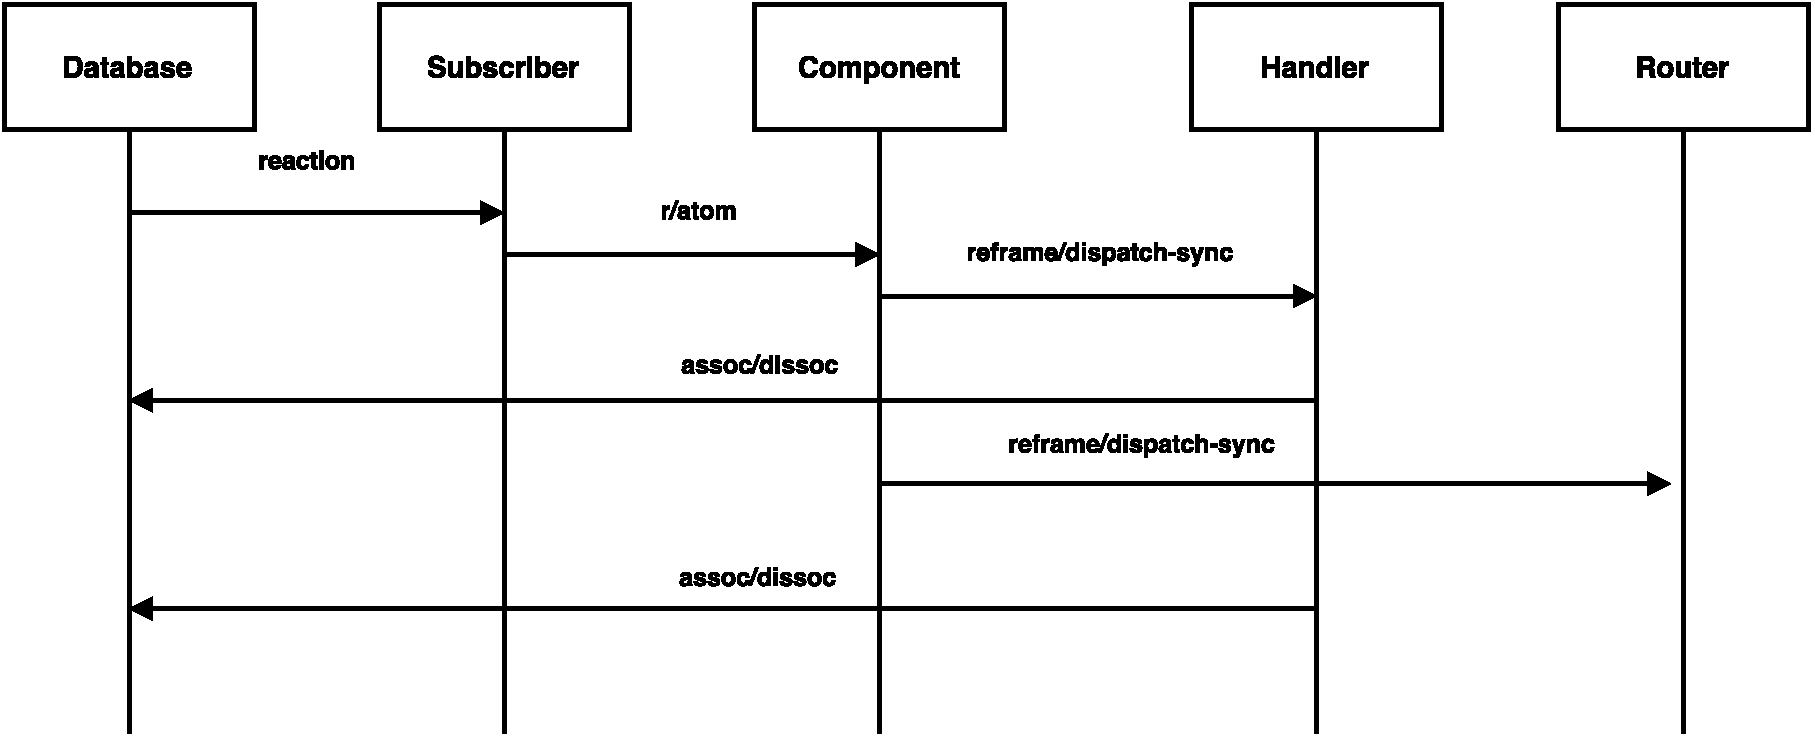
\includegraphics [width= \textwidth]{reframe_dataflow.pdf}
	\caption{Reframe, derived data flowing \cite{Reframe2016a}}
	\label{fig:reframe_dataflow}
\end{figure}




%%%%%%%%%%%%%%%%%%%%%%%%%%%%%%%%%%%%%%%%%%%%%%%%%%%%%%%%%%%%%%%%%%%%%%%%%
\subsection{Realization of Entity Views}
\label{subsec:realofentityviews}
%%%%%%%%%%%%%%%%%%%%%%%%%%%%%%%%%%%%%%%%%%%%%%%%%%%%%%%%%%%%%%%%%%%%%%%%%
The XML Schema Definition of entity type has been provided in \ref{lst:xsdlist}



\begin{Listing}
	\begin{lstlisting}
	<xs:complexType name="tEntityType" abstract="true">
	<xs:complexContent>
	<xs:extension base="tExtensibleElements">
	<xs:sequence>
	<xs:element name="Tags" type="tTags" minOccurs="0"/>
	<xs:element name="DerivedFrom" minOccurs="0">
	<xs:complexType>
	<xs:attribute name="typeRef" type="xs:QName" use="required"/>
	</xs:complexType>
	</xs:element>
	<xs:element name="PropertiesDefinition" minOccurs="0">
	<xs:complexType>
	<xs:attribute name="element" type="xs:QName"/>
	<xs:attribute name="type" type="xs:QName"/>
	</xs:complexType>
	</xs:element>
	</xs:sequence>
	<xs:attribute name="name" type="xs:NCName" use="required"/>
	<xs:attribute name="abstract" type="tBoolean" default="no"/>
	<xs:attribute name="final" type="tBoolean" default="no"/>
	<xs:attribute name="targetNamespace" type="xs:anyURI" use="optional"/>
	</xs:extension>
	</xs:complexContent>
	</xs:complexType>>
	\end{lstlisting}
	\caption{XML Schema Definition of Entity Type}
	\label{lst:xsdlist}
\end{Listing}

%%%%%%%%%%%%%%%%%%%%%%%%%%%%%%%%%%%%%%%%%%%%%%%%%%%%%%%%%%%%%%%%%%%%%%%%%
\subsection{Realization of Organizational Intentions}
%%%%%%%%%%%%%%%%%%%%%%%%%%%%%%%%%%%%%%%%%%%%%%%%%%%%%%%%%%%%%%%%%%%%%%%%%


%%%%%%%%%%%%%%%%%%%%%%%%%%%%%%%%%%%%%%%%%%%%%%%%%%%%%%%%%%%%%%%%%%%%%%%%%
\subsection{Realization of Organizational  Strategies}
%%%%%%%%%%%%%%%%%%%%%%%%%%%%%%%%%%%%%%%%%%%%%%%%%%%%%%%%%%%%%%%%%%%%%%%%%

%%%%%%%%%%%%%%%%%%%%%%%%%%%%%%%%%%%%%%%%%%%%%%%%%%%%%%%%%%%%%%%%%%%%%%%%%
\subsection{Realization of Organizational Capabilities}
%%%%%%%%%%%%%%%%%%%%%%%%%%%%%%%%%%%%%%%%%%%%%%%%%%%%%%%%%%%%%%%%%%%%%%%%%
There are two types of capabilities. Functional capabilities and cross-functional capabilities. Functional capabilities must be associated with instance descriptors. Cross-functional capabilities are capabilities containing multiple functional capabilities. We need to have the ability to add and remove instance descriptors for an entity type, e.g, resource definitions,  informal process definitions, etc. An instance descriptor of a functional capability should refer to a resource definition meaning that a capability is provided by a resource definition. So an instance descriptor of a capability refers to a resource definition and we can manually add and remove resource definitions in general.




%%%%%%%%%%%%%%%%%%%%%%%%%%%%%%%%%%%%%%%%%%%%%%%%%%%%%%%%%%%%%%%%%%%%%%%%%
\subsection{Realization of Organizational Resources}
%%%%%%%%%%%%%%%%%%%%%%%%%%%%%%%%%%%%%%%%%%%%%%%%%%%%%%%%%%%%%%%%%%%%%%%%%
You should have 2 keys one for tosca repository and one for tosca modeling tool. Tosca repo url refers to Winey and the other one refers to topology modeler. You should only contain root contexts and additional suffixes such as service templates in a separate key in default db.Out of these a function should create corresponding url for topology modeling.You can’t compute the topology modeler page of a specific service temple without knowing its id and namespace.You are trying to compose it from different variables: :topology-modeler-url, :tosco-repository-url,:target-namespace, and :id.


\fbox{\begin{minipage}{\textwidth}
		\{topology-modeler-url\}?repositoryURL=\{encoded-tosca-repository-url\}\&ns=\{encoded-target-namepsace\}\&id=\{encoded-id\}\#
	\end{minipage}}
	
	
	What important is, at the end what you should have a view that is capable of adding, viewing, deleting and updating models aligned with the XSD schema. In general, separate entities should reference each other but not contain each other. For instance, a strategy containing a goal should use goals id to resolve it but not the actual goal.
	
	
	%%%%%%%%%%%%%%%%%%%%%%%%%%%%%%%%%%%%%%%%%%%%%%%%%%%%%%%%%%%%%%%%%%%%%%%%%
	\subsection{Realization of Organizational Processes}
	%%%%%%%%%%%%%%%%%%%%%%%%%%%%%%%%%%%%%%%%%%%%%%%%%%%%%%%%%%%%%%%%%%%%%%%%%
	
	
	%%%%%%%%%%%%%%%%%%%%%%%%%%%%%%%%%%%%%%%%%%%%%%%%%%%%%%%%%%%%%%%%%%%%%%%%%
	\subsection{Realization of Informal Process Instances}
	%%%%%%%%%%%%%%%%%%%%%%%%%%%%%%%%%%%%%%%%%%%%%%%%%%%%%%%%%%%%%%%%%%%%%%%%%
	Informal process instances are separate entities similar to informal process models. They should be listed on the left side similar to informal process models. When one of the instance is selected by user, its properties should be presented on the right.
	
	
	
	
	
	%%%%%%%%%%%%%%%%%%%%%%%%%%%%%%%%%%%%%%%%%%%%%%%%%%%%%%%%%%%%%%%%%%%%%%%%%
	\subsection{Realization of Requirements}
	\label{subsec:realizationofrequirements}
	%%%%%%%%%%%%%%%%%%%%%%%%%%%%%%%%%%%%%%%%%%%%%%%%%%%%%%%%%%%%%%%%%%%%%%%%%
	
	\section{Validation and Evaluation}
	\label{sec:evaluation}
	%queries and print screens
	
	%%%%%%%%%%%%%%%%%%%%%%%%%%%%%%%%%%%%%%%%%%%%%%%%%%%%%%%%%%%%%%%%%%%%%%%%%
	\subsection{Validation of Components}
	\label{subsec:validationofcomponents}
	%%%%%%%%%%%%%%%%%%%%%%%%%%%%%%%%%%%%%%%%%%%%%%%%%%%%%%%%%%%%%%%%%%%%%%%%%
	
	
	
	
	%%%%%%%%%%%%%%%%%%%%%%%%%%%%%%%%%%%%%%%%%%%%%%%%%%%%%%%%%%%%%%%%%%%%%%%%%
	\subsection{Validation of Prototype}
	\label{subsec:validationofprototype}
	%%%%%%%%%%%%%%%%%%%%%%%%%%%%%%%%%%%%%%%%%%%%%%%%%%%%%%%%%%%%%%%%%%%%%%%%%
	
	


